\documentclass[11pt]{article}
\usepackage[margin=0.5in]{geometry}
\usepackage{graphicx}
\usepackage{amsmath}
\usepackage{enumitem}

\graphicspath{{/home/konner/Pictures/} }
\begin{document}
\centerline{\Large Stats 170, Homework 1}
\vspace{.5pc}
\centerline{\Large Konner Macias - 004603916}
\vspace{1.5pc}
\section{}
c) 
\begin{center}
	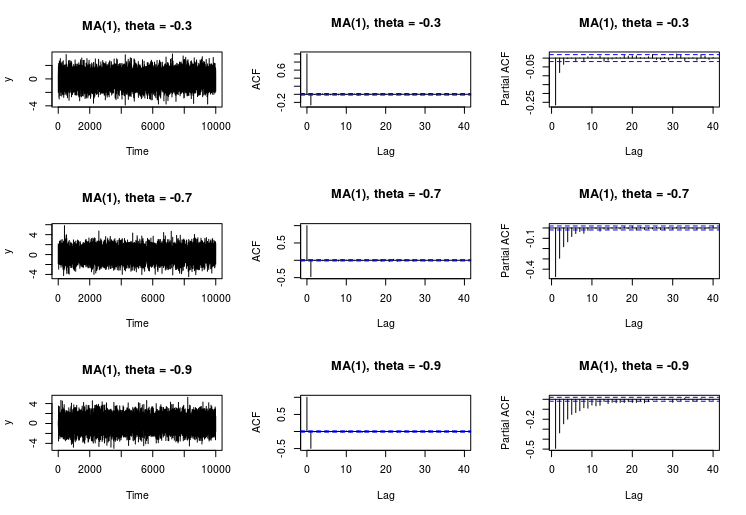
\includegraphics[scale=1]{plt1.png}
\end{center}

\newpage
d) The time plot appears to fluctuate randomly around zero no matter how large the negative coefficient grows in asbolute value. Even upon inspection using the window() function, the time plots appear to remain the same, with the amplitudes all remaining similar. The ACF appears to remain constant across all magnitudes of theta, with only lag 1 being significant. However, more lags become significant in the partial correlogram as theta increases in terms of absolute value. The partial ACF values appear to be mainly negative.   
\\\\
e) The three timeplots share the fact that they each fluctuate randomly around zero. The ACFs appear to remain constant across all values of theta. The PACFs share the fact that the first few lags, no matter the theta value, are significant.  
\\\\
f)  The ACFs do not have any major differences besides that the autocorrelation values are increasing in terms of absolute value as theta increases in terms of absolute value, and share the pattern of lag 1 being significant. The PACFs follow a visual pattern as the value of theta decreases. There seems to be more statistically significant partial auto correlations (more lags) for larger values of theta in terms of absolute value as demonstrated in the PACFs. 
\\\\
g) Across all plots, lag 1 is significant. We achieve an autocorrelation values of $-0.265, -0.472, -0.492$ for $\theta = -0.3, \theta = -0.7, \theta = -0.9$, respectively. 
\\\\
h) The three autocorrelations values are ${-0.265}$, ${-0.472}$, ${-0.492}$ for theta $ = -0.3,-0.7,-0.9$, respectively. We can double check that the theoretical relation between the model formula and the autocorrelations holds. Given the formula for rho, $$ \rho_1 =  \frac{\theta_1}{1 + \theta_1^2} $$ Let's now rearrange to solve for $\theta$. 

$$ \rho_1 \theta_1^2 - \theta_1 + \rho_1 = 0 $$
$$ \theta_1 = \frac{1 - \sqrt{1-4\rho_1^2}}{2\rho_1} $$
 
For $\rho = -0.265$, we achieve:
$$ \theta_1 = \frac{1 - \sqrt{1-4(-0.265)^2}}{2(-0.265)} $$
$$ \theta_1 \approx -0.3 $$

For $\rho = -0.472$, we achieve:
$$ \theta_1 = \frac{1 - \sqrt{1-4(-0.472)^2}}{2(-0.472)} $$
$$ \theta_1 \approx -0.7 $$

For $\rho = -0.492$, we achieve:
$$ \theta_1 = \frac{1 - \sqrt{1-4(-0.492)^2}}{2(-0.492)} $$
$$ \theta_1 \approx -0.9 $$

\newpage
\section{}
Given that lag $k = 1$ of an MA(1) process equals $\rho_1 = 0.4$, we can estimate the slope parameter using $$ \beta_1 = \frac{1 -\sqrt{1-4 \rho_1^2}}{2 \rho_1} $$  $$ \beta_1 = \frac{1-\sqrt{1-4 (0.4)^2}}{2(0.4)} $$
$$ \beta_1 = \frac{1}{2} $$. The corresponding MA(1) model is $$ Y_t = \epsilon_t + \frac{1}{2}\epsilon_{t-1} $$ where $\epsilon_t$ is white noise. Since this is an MA(1) process, to satisfy a theoretical restriction called invertibility, MA(1) models must have values with absolute value less than 1.\\\\
Source: https://onlinecourses.science.psu.edu/stat510/node/48/.
\newpage


\section{}
Determine whether the following process is first or second order stationary. $$ y_t = 5 + w_t - \frac{1}{2}w_{t-1} + \frac{1}{4}w_{t-2} $$.

Expectation:
$$ E[y_t] = E(5) + E(w_t) - E(\frac{1}{2}w_{t-1}) + E(\frac{1}{4}w_{t-2}) $$
$$ E[y_t] = 5 + E(w_t) - \frac{1}{2}E(w_{t-1}) + \frac{1}{4}E(w_{t-2}) $$
$$ E[y_t] = 5 + 0 + 0 + 0 = 5 $$

Variance:
$$ Var[y_t] = var(5) + var(w_t) - var(\frac{1}{2}w_{t-1}) + var(\frac{1}{4}w_{t-2}) $$
$$ Var[y_t] = var(5) + var(w_t) + \frac{1}{4}var(w_{t-1}) + \frac{1}{16}var(w_{t-2}) $$
$$ Var[y_t] = \sigma^2 + \frac{1}{4}\sigma^2 + \frac{1}{16}\sigma^2 = \frac{21}{16}\sigma^2 $$

Autocovariance:
$$ Cov(y_t, y_{t-1}) = E[(w_t - \frac{1}{2}w_{t-1} + \frac{1}{4}w_{t-2})(w_{t-1} - \frac{1}{2}w_{t-2} + \frac{1}{4}w_{t-3})] = \gamma_1 $$
$$ \Rightarrow E[w_t w_{t-1} - \frac{1}{2}w_t w_{t-2} + \frac{1}{4}w_t w_{t-3} + $$
$$ -\frac{1}{2}w_{t-1}^2 + \frac{1}{4}w_{t-1} w_{t-2} - \frac{1}{8}w_{t-1}w_{t-3} + $$
$$ \frac{1}{4} w_{t-2}w_{t-1} - \frac{1}{8}w_{t-2}^2 + \frac{1}{16}w_{t-2} w_{t-3} ] $$

$$ \Rightarrow Cov(w_t, w_{t-1}) - \frac{1}{2}Cov(w_t ,w_{t-2}) + \frac{1}{4}Cov(w_t,w_{t-3}) + $$
$$ -\frac{1}{2}E(w_{t-1}-0)^2 + \frac{1}{4}Cov(w_{t-1}, w_{t-2}) - \frac{1}{8}Cov(w_{t-1},w_{t-3}) + $$
$$ \frac{1}{4} Cov(w_{t-2},w_{t-1}) - \frac{1}{8}E(w_{t-2}-0)^2 + \frac{1}{16}Cov(w_{t-2},w_{t-3}) $$

$$ \Rightarrow \gamma_1 = -\frac{1}{2}\sigma^2 - \frac{1}{8}\sigma^2 = -\frac{5}{8}\sigma^2$$

Thus, lag 1 is: 
$$ \rho_1 = \frac{-\frac{1}{2} - \frac{1}{8}}{\frac{21}{16}} = -\frac{10}{21} $$

Following the same process for $\gamma_2$, we earn:
$$ Cov(y_t, y_{t-2}) = \frac{1}{4}\sigma^2 = \gamma_2 $$
This, lag 2 is:
$$ \rho_2 = \frac{\frac{1}{4}}{\frac{21}{16}} = \frac{4}{21} $$

This process is a second order process, since:
$$ E[y_t] = 5 = \mu $$
$$ Var[y_t] = \frac{21}{16}\sigma^2 = (1 + \beta_1^2 + \beta_2^2) \sigma^2 $$
ACF
$$ \rho_1 = \frac{-\frac{1}{2} - \frac{1}{8}}{\frac{21}{16}} = \frac{\beta_1 + \beta_1 \beta_2}{1 + \beta_1^2 + \beta_2^2} $$
$$ \rho_2 = \frac{\frac{1}{4}}{\frac{21}{16}} = \frac{\beta_2}{1 + \beta_1^2 + \beta_2^2} $$
$$ \rho_k = 0 \text{ for all } k > 2$$

with $\beta_1 = -\frac{1}{2}$ and $\beta_2 = \frac{1}{4}$. \\\\
This is not an order one process as the second lag is nonzero. Since it satisfies all the properties of a second-order process, it must be one itself.

\newpage
\section{}
a)   
\begin{center}
	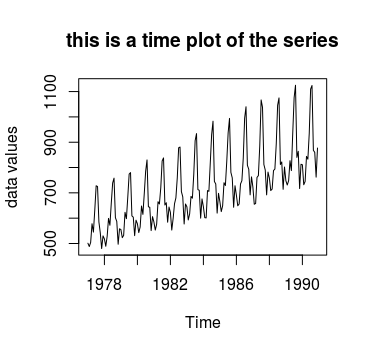
\includegraphics[scale=1]{plt4a}    
\end{center}

We notice that there is strong seasonality, and an upwards trend with no obvious outliers. The range of the seasons is very small.  
  
c)  
\begin{center}
	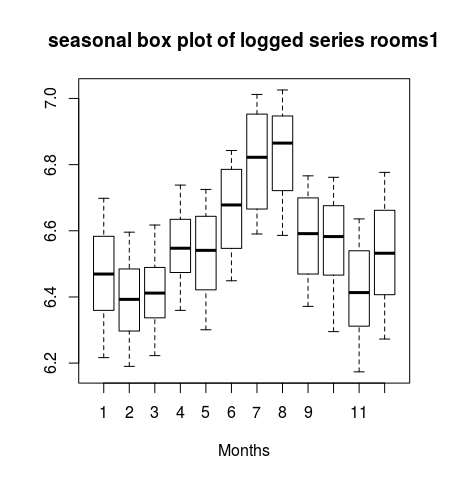
\includegraphics[scale=.9]{plt4c}  
\end{center}
During the summer months of July and August, we notice higher numerical value, as their median of the boxplot is higher than the others. The trend to be the shape of a bell curve with its peak being the summer months. Thus, in terms of its seasonality, we will expect peaks in values during the summer times of each year.  
\\\\
d)  
\begin{center}
	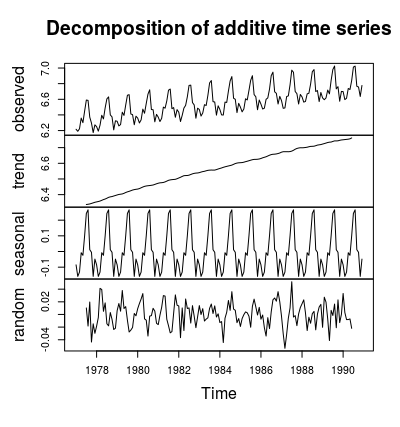
\includegraphics[scale=1]{plt4d}
\end{center}
  
Within this additive decomposition plot, first within the oberserved plot, we notice that there is an upwards trend with seasonality and no obvious outleirs. The next plot, trend, nearly grows linearly in the positive direction. The seasonal plot is perfectly constructed as we notice the repeating pattern. Lastly, the random plot does appear stationary with no obvious trends, nearly like white noise.  
\\
f)  
\begin{center}
	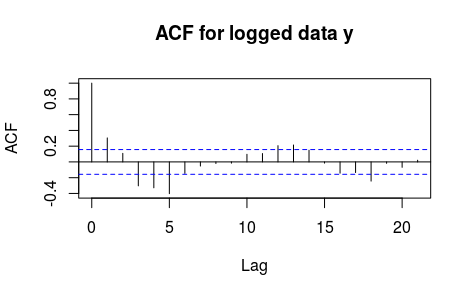
\includegraphics[scale=1]{plt4f1}
	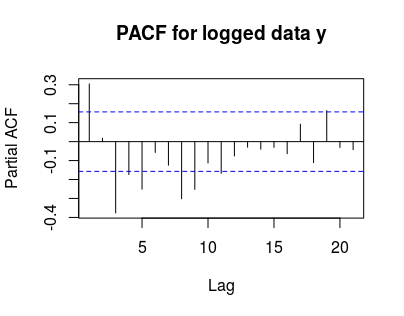
\includegraphics[scale=1]{plt4f2}
\end{center}

We notice that lags 1,3,4,5,12,13, and 18 are statistically significant in the ACF achieving values of $0.304, -0.303, $ \\
$ -0.328, -0.402, 0.206, 0.215, -0.243$, respectively. Because of the typo in this question, we can either be comparing MA(1) and MA(2) or we can compare MA(1) and AR(1). In either circumstance, the model generating this time series is neither of these options. \\\\

For an AR(1) model, we would expect the ACF to exponentially decrease to 0 as the lag increases, but this ACF fluctuates back and forth. While the PACF is geometric, indicating an MA(1) possibility, it is however not true as we would expect for the ACF to only have a significant autocorrelation at lag 1 for an MA(1). This instance has several lags that have proved significant. Similarly, for an MA(2), we would expect only 2 lags that are statistically significant but we are achieving 7 in this instance.
\\\\
g)  
\begin{center}
	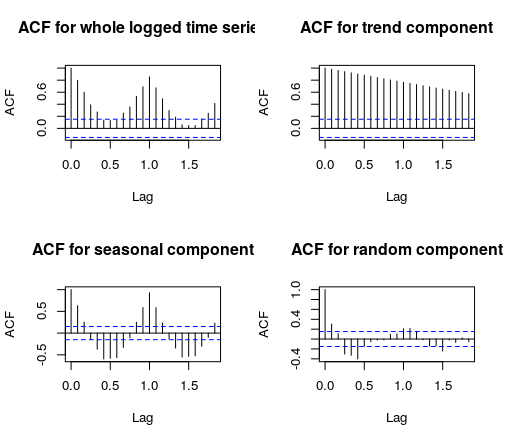
\includegraphics[scale=1]{plt4g}
\end{center}


\newpage
\section{}
a)
\begin{center}
	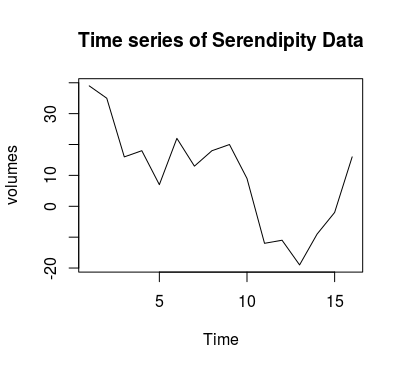
\includegraphics[scale=1]{plt5a1}
	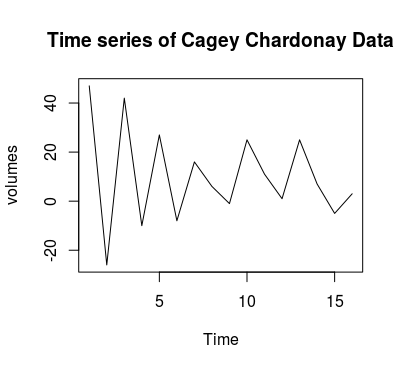
\includegraphics[scale=1]{plt5a2}
\end{center}

First off, we notice that the Cagey Chardonay has some seasonality or periodicity as it fluctuates in a pattern. It tends to fluctuate close to zero. The Serendipity data does not fluctuate nearly as often and is composed on an overall downwards trend, with a downwards trend for the first 13 time steps and an upwards trend for the latter time steps.  
\\\\
b)
\begin{center}
	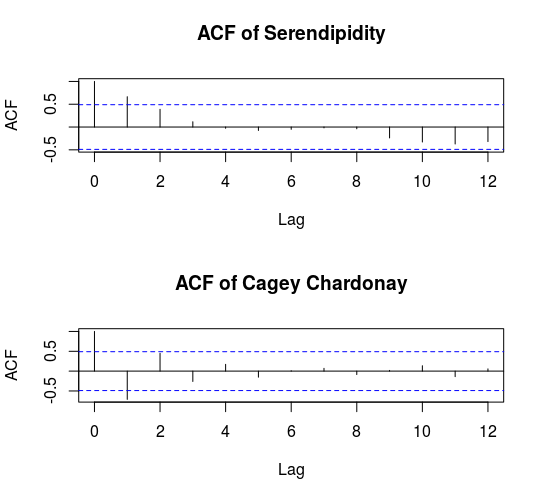
\includegraphics[scale=1]{plt5b}
\end{center}

For both ACFs, we notice that only lag 1 is statistically significant. For Serendipity, we notice the ACF has more a gradual decay, implying an AR(1) process. For Cagey Chardonnay, we see that the ACF is significant only one lag without a gradual decay, it is most likely an MA(1) process.
\\\\
c) If I were a wine retailer, I would trust the Cagey Chardonnay vineyard. The Serendipity vineyard largely showcases a downward trend, an since it is an AR(1) process, it is not always stationary. Cagey Chardonnay is more reliable as it is stationary and consistently fluctuates near zero.

\end{document}